\documentclass[../TDM1-M2.tex]{subfiles}%

\begin{document}
\section[s]"2"{Coup franc et frottements fluides}

\enonce{%
	\noindent
	\begin{minipage}{0.45\linewidth}
		On étudie dans le référentiel terrestre galiléen de repère fixe (O,$x$,$y$),
		un coup franc de football tiré à \SI{20}{m}, face au but de hauteur
		\SI{2,44}{m} et dans son plan médian vertical ($x$O$y$). L'axe (O$y$) est
		choisi suivant la verticale ascendante.
	\end{minipage}
	\hfill
	\begin{minipage}{0.45\linewidth}
		\begin{center}
			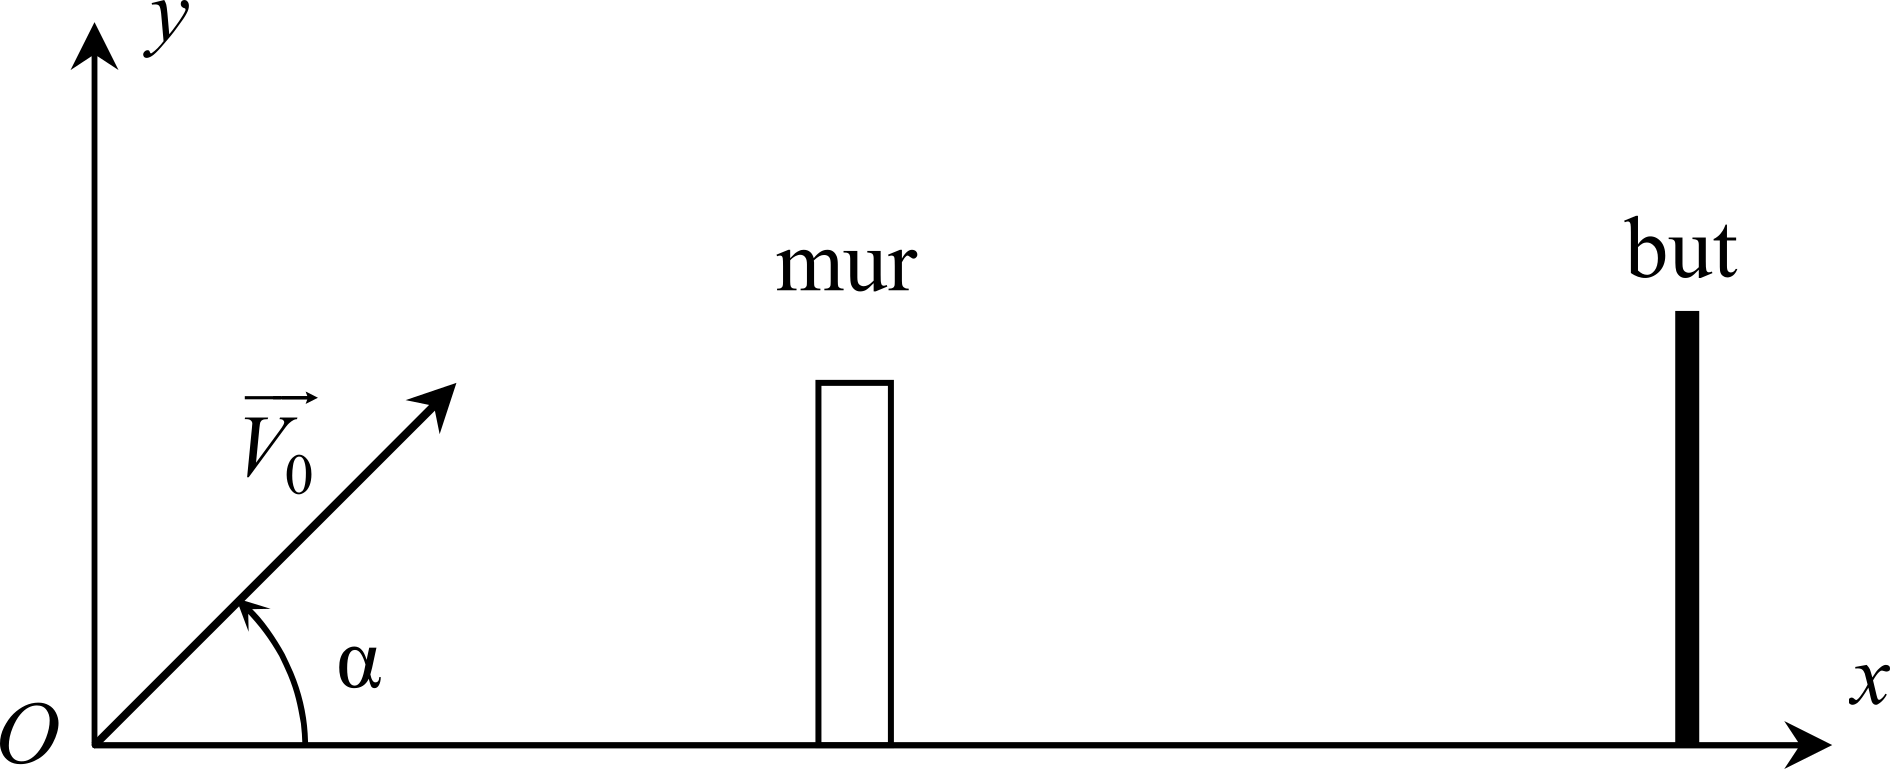
\includegraphics[width=\linewidth]{coup_franc-plain}
		\end{center}
	\end{minipage}
	\smallbreak
	Le ballon, de masse $m = \SI{430}{g}$, est assimilé à un point matériel M
	initialement au sol en O. Le mur, de hauteur \SI{1,90}{m}, est situé à
	\SI{9,15}{m} du ballon. Le ballon est lancé à l'instant $t = 0$ avec une vitesse
	initiale $v_0$ de norme \SI{20}{m.s^{-1}} et formant un angle $\alpha$ de
	\ang{20;;} avec l'horizontale. On note $g$ l'accélération de la pesanteur et on
	rappelle que $g = \SI{9,81}{m.s^{-2}}$.
}

\begin{blocQR}
	\item Dans un premier temps, on néglige totalement les frottements de l'air.
	\QR{%
		Établir les équations horaires du mouvement du ballon ainsi
		que l'équation de la trajectoire.
	}{%
		~
		\vspace{-15pt}
		\smallbreak
		\begin{itemize}
			\item[b]{Système}~: \{ballon\}
			\item[b]{Référentiel}~: terrestre galiléen
			\item[b]{Repère}~: cartésien $(\Or,\ux,\uy)$, $\uy$ vertical
			      ascendant, $\ux$ vers le but
			\item[b]{Repérage}~: $\OM(t) = x(t)\ux + y(t)\uy$, $\vf(t) = \xp(t)\ux +
				      \yp(t)\uy$, $\af(t) = \xpp(t)\ux + \ypp(t)\uy$
			\item[b]{Origine et instant initial}~: $\OM(0) = \of$
			\item[b]{Vitesse initiale}~: $\vf(0) = v_0\cos\a\ux +
				      v_0\sin\a\uy$
			\item[b]{BDF}~:
			      \[
				      \begin{array}{ll}
					      \textbf{Poids} & \Pf = m\gf = -mg\uy
				      \end{array}
			      \]
			\item[b]{PFD}~:
			      \begin{gather}
				      \label{eq:foot1pfd}
				      \cancel{m}\af = -\cancel{m}g\uy
				      \Lra
				      \left\{
				      \begin{array}{rcl}
					      \xpp & = & 0  \\
					      \ypp & = & -g
				      \end{array}
				      \right.
			      \end{gather}
		\end{itemize}
		Ainsi,
		\begin{gather}
			\label{eq:foot1eqho}
			\eqref{eq:foot1pfd}
			\Ra
			\left\{
			\begin{array}{rcl}
				\xp & = & v_0\cos\a       \\
				\yp & = & -gt + v_0\sin\a
			\end{array}
			\right.
			\Ra
			\left\{
			\boxed{
				\begin{aligned}
					x(t) & = v_0t\cos\a                    \\
					y(t) & = -\frac{1}{2}gt^2 + v_0t\sin\a
				\end{aligned}
			}
			\right.
		\end{gather}
		étant donné les conditions initiales. On trouve la
		trajectoire en isolant $t(x)$ pour avoir $y(x)$~:
		\begin{gather*}
			\eqref{eq:foot1eqho}
			\Ra
			\left\{
			\begin{aligned}
				t(x) & = \frac{x}{v_0\cos\a}               \\
				\Aboxed{
				y(x) & = - \frac{g}{2v_0{}^2\cos^2\a}x^2 +
				x\tan\a}
			\end{aligned}
			\right.
		\end{gather*}
	}
	\QR{%
		Le ballon passe-t-il au-dessus du mur~?
	}{%
		Le ballon passe au-dessus du mur si $y(x\ind{mur}) \geq
			h\ind{mur}$ avec $h\ind{mur}$ la hauteur du mur et $x\ind{mur}$
		sa position horizontale. Avec une application numérique, on
		obtient
		\[y(x\ind{mur}) = \SI{2.17}{m} > h\ind{mur} = \SI{1.90}{m}\]
		donc le ballon \underline{passe bien au-dessus du mur}.
	}

	\QR{%
		Le tir est-il cadré~?
	}{%
		Le tir est cadré si $y(x\ind{but}) \leq h\ind{but}$. Or,
		\[y(x\ind{but}) = \SI{1.73}{m}\]
		donc \underline{le tir est bien cadré}.
	}

	\item Il y a en réalité des frottements, modélisés par une force $\Fff =
		-\alpha\vf(t)$ avec $\alpha = \SI{5.00e-3}{kg.s^{-1}}$.
	\resetQ
	\QR{%
		Déterminer les équations horaires en introduisant la constante
		$\tau = \frac{m}{\alpha}$.
	}{%
		Avec le même système, seul le bilan des forces est modifié (et
		donc le PFD)~:
		\begin{itemize}
			\item[b]{BDF}~:
			      \[
				      \begin{array}{ll}
					      \textbf{Poids}       & \Pf = -mg\uy                        \\
					      \textbf{Frottements} & \Ff = -\alpha\vf(t) = -\alpha\xp\ux
					      -\alpha\yp\uy
				      \end{array}
			      \]
			\item \leftcenters{\bfseries
				      PFD}~:{$m\af = -mg\uy -\alpha\xp\ux -\alpha\yp\uy$}
		\end{itemize}
		\vspace{-10pt}
		\begin{align*}
			\Lra
			\left\{
			\begin{aligned}
				m\xpp & = -\alpha\xp     \\
				m\ypp & = -mg -\alpha\yp
			\end{aligned}
			\right.
			 & \Lra
			\left\{
			\begin{aligned}
				\xpp + \frac{\alpha}{m}\xp & = 0  \\
				\ypp + \frac{\alpha}{m}\yp & = -g
			\end{aligned}
			\right.
			\\\Lra
			\left\{
			\begin{aligned}
				\dot{v_x} + \frac{v_x}{\tau} & = 0  \\
				\dot{v_y} + \frac{v_y}{\tau} & = -g
			\end{aligned}
			\right.
			 & \Lra
			\left\{
			\begin{aligned}
				v_x(t) & = A\exr^{-t/\tau}          \\
				v_y(t) & = -g\tau + B\exr^{-t/\tau}
			\end{aligned}
			\right.
			\\
			\text{Or,}\quad
			\left\{
			\begin{aligned}
				v_x(0) & = v_0\cos\a \\
				v_y(0) & = v_0\sin\a
			\end{aligned}
			\right.
			 & \Ra
			\left\{
			\begin{aligned}
				A & = v_0\cos\a         \\
				B & = v_0\sin\a + g\tau
			\end{aligned}
			\right. \\
			\text{donc}\quad
			\left\{
			\begin{aligned}
				v_x(t) & = v_0\cos\a\exr^{-t/\tau} \\
				v_y(t) & = \left(v_0\sin\a
				+ g\tau\right)\exr^{-t/\tau}
				-g\tau
			\end{aligned}
			\right.
			 & \Ra
			\left\{
			\begin{aligned}
				x(t) & = -v_0\tau\cos\a\exr^{-t/\tau}
				+ C                                   \\
				y(t) & = -\left(v_0\tau\sin\a
				+ g\tau^2\right)\exr^{-t/\tau}
				-g\tau t + D
			\end{aligned}
			\right. \\
			\qor
			\left\{
			\begin{aligned}
				x(0) & = 0 \\
				y(0) & = 0
			\end{aligned}
			\right.
			 & \Ra
			\left\{
			\begin{aligned}
				C & = v_0\tau\cos\a                         \\
				D & = +\left(v_0\tau\sin\a + g\tau^2\right)
			\end{aligned}
			\right.
		\end{align*}
		Finalement,
		\begin{empheq}[box=\fbox, left=\empheqlbrace]{align}
			\label{eq:foot2x}
			x(t) &= v_0\tau\cos\a\left(1 - \exr^{-t/\tau}\right)\\
			\label{eq:foot2y}
			y(t) &= \left(v_0\tau\sin\a + g\tau^2\right)
			\left(1-\exr^{-t/\tau}\right) -g\tau t
		\end{empheq}
	}
	\QR{%
		Donner l'équation de la trajectoire.
	}{%
		On isole $t(x)$ de \eqref{eq:foot2x} pour l'injecter dans
		\eqref{eq:foot2y}~:
		\begin{empheq}[box=\fbox, left=\empheqlbrace]{align*}
			% \label{eq:foot2t}
			t(x) &= -\tau\ln(1- \frac{x}{v_0\tau\cos\a})\\
			% \label{eq:foot2traj}
			y(x) &= \left(\tan\a + \frac{g\tau}{v_0\cos\a}\right)x
			+g\tau^2\ln(1- \frac{x}{v_0\tau\cos\a})
		\end{empheq}
	}
	\QR{%
		Le ballon passe-t-il au-dessus du mur~?
	}{%
		On calcule~:
		\[y(x\ind{mur}) = \SI{2.16}{m}\]
		donc \underline{le ballon passe au-dessus du mur}.
	}
	\QR{%
		Le tir est-il cadré~?
	}{%
		On calcule~:
		\[y(x\ind{but}) \approx \SI{1.68}{m}\]
		donc \underline{le tir est bien cadré}. On constate que les
		frottements n'ont eu que peu d'influence sur ce mouvement~; il
		n'est en effet pas très rapide, donc la force de frottements est
		restée assez faible.
	}
\end{blocQR}

\end{document}
